\chapter{Entity and mapping translation}\label{chapter:entity_translation}
% what is all needed (+table comparison)
% abstraction and wrappers (generally)
% algorithm pseudocodes - builder+ parser for mappings, visitor for queries
% working with the abstract classes, not concrete implementation
% concrete example dapper -> something complex (NH/EF)
% all theory - no limit of implementation (DB querying is present etc)
% special cases

The chapter begins by examining entities and their database mapping. Although the frameworks analyzed earlier differ in syntax and configuration approaches, they nonetheless share several common patterns. The aim of this chapter is to identify these common concepts and to design a unified abstraction. This abstraction should be expressive enough to capture all mapping capabilities while remaining independent from any specific implementation. Once the abstraction is defined, algorithms that support its translation can be developed.

\section{Abstraction for translation}\label{sec:def_abstract}

Beginning, with the entity, at its core, it is a plain C\# class composed of properties. Typically, such a class corresponds to a single database table, with each property representing a directly loaded or transformed column value. The mapping must describe this relationship explicitly. In many cases, class and property names serve as defaults, but when they diverge from their database identifiers, aliases must be specified. The .NET type system does not fully align with that of database systems. While the property's type and nullability often provide sufficient hints, more specific constraints -- such as length, precision, or character encoding -- require explicit configuration.

And of course, a table rarely exists in isolation. In a relational model, it is typically connected to others through defined relationships. The mapping must at least capture primary and foreign keys to allow proper navigation. More complex associations often require further configuration. An \acrshort{orm} may need to know which side owns the relationship, how cascading behaviour is handled, or how orphaned entities are treated.

It is worth noting that features operating purely on the database side such as indexes, triggers, or computed columns are generally outside the scope of entity mapping. Some \acrshort{orm}(s)\footnote{\url{https://learn.microsoft.com/en-us/ef/core/modeling/indexes}, \url{https://learn.microsoft.com/en-us/ef/core/modeling/generated-properties}} allow limited representation of those features, but they are not considered in the abstraction.

The Table~\ref{tab:entity_mapping} is a result of framework examination in Chapter~\ref{chapter:ormcomparison}. First, important parts of entity mapping were identified, each represented by a table row. Each column depicts a different \acrshort{orm} and how the specific mapping is implemented. All possible mapping formats are not considered, and those selected in Section~\ref{sec:perf_eval} are used. 

From the table rows, it is evident that the most important mapping concepts include \textbf{table} and \textbf{schema names}, the names, types, and nullability of \textbf{columns}, as well as column \textbf{constraints} such as length, scale, and precision. Furthermore, \textbf{primary keys} with their respective strategies for generation and \textbf{foreign keys} along with their cardinalities emerged as significant factors for relationships.

%\clearpage
\afterpage{
\begin{landscape}
\begin{table}[p]
\centering
\caption{Comparison of key mapping aspects across different frameworks.}
\label{tab:entity_mapping}
\scriptsize
\def\arraystretch{1.75}
\begin{tabular}{
>{\raggedright\arraybackslash}p{27.00mm}
>{\arraybackslash}p{29.00mm}
>{\arraybackslash}p{29.00mm}
>{\arraybackslash}p{30.00mm}
>{\arraybackslash}p{29.50mm}
>{\arraybackslash}p{38.00mm}
>{\arraybackslash}p{35.00mm}
}
\toprule
  &    \textbf{Dapper}\newline no mapping &  \textbf{PetaPoco} \newline attribute mapping &    \textbf{RepoDB} \newline attribute mapping &   \textbf{LINQ to DB} \newline fluent mapping & \textbf{NHibernate} \newline \acrshort{xml} file mapping  &   \textbf{EF Core} \newline attribute mapping \\
\midrule
\textbf{Primary key}  & - & \texttt{[PrimaryKey]} on class & \texttt{[Primary]} on property & HasPrimaryKey() & \texttt{<id name="OrderID" column="" type="">\ldots</id>} & \texttt{[Key]} on property \\

%\midrule
\textbf{Foreign key} & – & – & – & \texttt{.Association()}  & in \texttt{one-to-many} & \texttt{[ForeignKey]} \\

%\midrule
\textbf{Table and schema} &
– &
\texttt{[TableName("x.y")]} &
\texttt{[Table("y", Schema="x")]} &
\texttt{.HasSchemaName("x")} \newline \texttt{.HasTableName("y")} &
\texttt{<class table="y" schema="x">} &
\texttt{[Table("y", Schema="x")]} \\

%\midrule
\textbf{Database type} & derived from property & derived from property & \texttt{[DbType]} & \texttt{.HasDbType()} & \texttt{type="decimal"} & \texttt{[Column(TypeName="")]} \\

%\midrule
\textbf{Precision} & – & – & \texttt{[Precision]} & \texttt{.HasPrecision()} & \texttt{precision="18" scale="2"} & \texttt{[Precision(18,2)]} \\

%\midrule
\textbf{Nullability} & derived from property & derived from property & \texttt{[IsNullable(true)]} & \texttt{.IsNullable()} & \texttt{not-null="false"} & derived from property \\

%\midrule
\textbf{One-to-one} & – \newline (join + \texttt{splitOn}) & – \newline (join + \texttt{Fetch<T1,T2>}) & – \newline (\texttt{QueryMultiple}) & \texttt{.Association()} \newline and mapped keys & \texttt{<bag> <key column=""/> <one-to-one class="" column=""/> </bag>} & mapped keys and derived from property type \\

%\midrule
\textbf{One-to-many} & – \newline (join + \texttt{splitOn}) & – \newline (join + \texttt{Fetch<T1,T2>}) & – \newline (\texttt{QueryMultiple}) & \texttt{.Association()} \newline and mapped keys & \texttt{<bag> <key column=""/> <one-to-many class="" column=""/> </bag>} & mapped keys and derived from property type \\

%\midrule
\textbf{Many-to-many} & – \newline (join + \texttt{splitOn}) & – \newline (join + \texttt{Fetch<T1,T2>}) & – \newline (raw SQL + in memory) & \texttt{.Association()} \newline and mapped keys  & \texttt{<bag> <key column=""/> <many-to-many class="" column=""/> </bag>} & fluent join-table definition:\newline\texttt{UsingEntity("", l => l.$\cdots$, r => r.$\cdots$)} \\
\bottomrule
\end{tabular}
\end{table}
\end{landscape}
}

\section{Intermediate representation}
%diagram fo design and specific parts
Building on the mapping aspects identified above, a unified intermediate representation can be proposed. The complete conceptual model is illustrated in the class diagram (\acrshort{uml}) in Figure~\ref{fig:abstract_ir}. This abstraction captures both application-level and database-level details of entity mapping in a structured and extensible manner. 

\begin{figure}[ht]
  \centering
  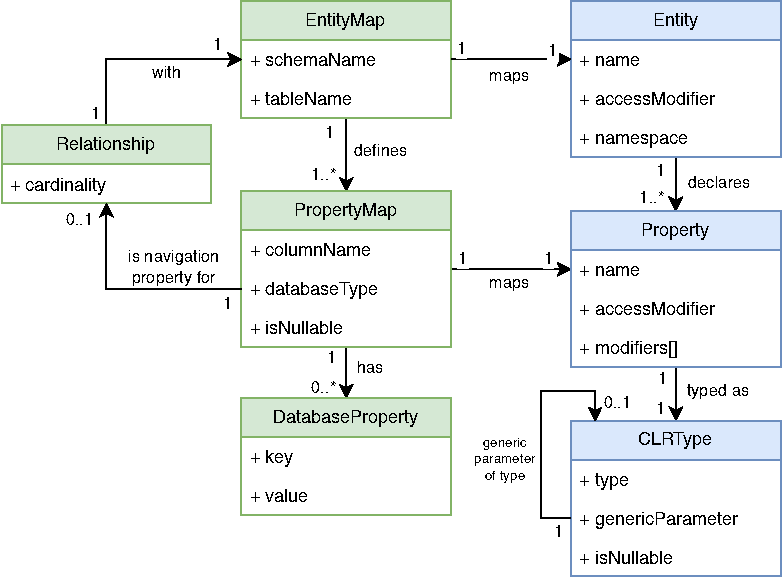
\includegraphics[scale=1]{thesis/img/thesis/03_abstract_ir.drawio.pdf}
  \caption{Class diagram of intermediate representation of entity mapping.}
  \label{fig:abstract_ir}
\end{figure}

The starting point for mapping is the representation of a C\# class itself, encapsulated in the \texttt{Entity} class. This class holds information about the entity's name, its access modifiers, and namespace. Additionally, the \texttt{Entity} references all individual properties it contains. Each property is represented using the \texttt{Property} class, which includes its access modifiers, data type, and name. 

Type information is extracted into the \texttt{CLRType} class (\acrshort{clr} referring to \acrlong{clr}) to allow nesting in a generic parameter. Such generics commonly appear in navigation properties for relationships, as .NET typically represents one-to-many or many-to-many relationships by collections (e.g. \texttt{List} or \texttt{HashMap}) parameterized by the target entity type. The classes \texttt{Entity}, \texttt{Property} and \texttt{CLRType} collectively represent the application-level aspects of the entity.

Additional classes must be introduced for database mapping purposes. At the core of data mapping representation is the \texttt{EntityMap} class, which acts as the primary container linking an entity class to a specific database table, namely schema and table names. Each entity property is mapped separately to its corresponding database column through the class \texttt{PropertyMap}, which stores details such as column name and its associated database data type.

When an entity property represents a foreign key, additional details about the cardinality and the target entity of the relationship must also be stored. These details are explicitly handled by the \texttt{Relationship} class. Additionally, the more complex features of column mapping, such as type constraints and other specialized attributes, are represented using the flexible \texttt{DatabaseProperty} class. This class maintains information in key-value pairs. For example, a decimal property type like \texttt{DECIMAL(15,8)} would be represented by  keys ``Precision'' and ``Scale'', holding values 15 and 8, respectively. And the base type ``decimal'' would go under \texttt{database type}. 

%The relationship between EntityMap and Entity has $1 \rightarrow 1$ multiplicity, but it could be modified to $1 \rightarrow *$ in the rare case of one entity mapping multiple tables.


\section{Translation}

With the intermediate representation model designed, translations in both directions are required. In one direction, a \textit{parser} processes the source entity and its mapping. And in the other direction, a \textit{builder} generates the target framework entity from the intermediate representation. This process is illustrated in Figure~\ref{fig:translation_process} and consists of two distinct phases: parsing and building.

To enforce separation of concerns, the intermediate representation resides within the builder, while the parser populates it by invoking methods defined in an abstract base class. Although concrete implementations are used during execution, they are accessed exclusively through the base interface or abstract class to maintain full decoupling.

\begin{figure}[ht]
  \centering
  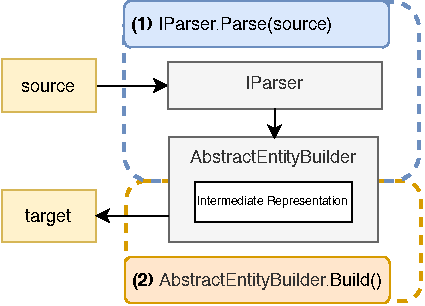
\includegraphics[scale=1]{thesis/img/thesis/03_translate_process.drawio.pdf}
  \caption{Translation process of entity with (1) parsing and (2) building phase.}
  \label{fig:translation_process}
\end{figure}

\subsection{Entity and mapping builder}

The builder accepts entity and mapping information through a common interface and constructs the intermediate representation, which it stores internally. Once the parsing phase is complete and the representation is fully populated, the builder proceeds to generate the target source code.

Since the target frameworks differ significantly in mapping styles, supported features, and default behaviours, each framework requires its own dedicated builder. Despite these differences, the process of constructing the intermediate representation is consistent across frameworks. To support this, all builders inherit from a shared abstract base class, \texttt{\textbf{AbstractEntityBuilder}}. It defines the common interface and core methods. And each concrete builder then implements the logic specific to generating syntax for its target framework.

The abstraction builds on the common concepts identified in Section~\ref{sec:def_abstract} and defines the following core methods. To support seamless replacement of an existing entity, the builder stores the class namespace via the \texttt{\textbf{AddNamespace}} method, enabling the generated code to be placed back into its original file (assuming new \acrshort{orm} is installed). The \texttt{\textbf{AddClassHeader}} captures the class name along with its access modifier. 
Schema and table names are handled separately from class-level metadata through \texttt{\textbf{AddSchema}} and \texttt{\textbf{AddTable}} methods, as their placement may differ across source frameworks. Together, these methods provide coverage for class and table-related metadata. 

The central method for defining class properties is \texttt{\textbf{AddProperty}}, which supports a wide range of (mostly optional) parameters. At minimum, it requires the property type and name. Additional parameters include modifiers, flags like \texttt{required} or \texttt{virtual}, nullability, default value, and getter/setter information. 

The database mapping counterpart for this method is provided by method \texttt{\textbf{AddPropertyMapping}}. It takes the property name and a hash map of column attributes. These attributes may include data type, length, scale, precision, and any other column-specific metadata. The use of hashmap provides flexibility in representing various column configurations. However, to ensure consistency, attribute keys must be standardized across all parser implementations -- either through documentation or shared statically typed constants.

To define relationships, two methods are available for handling primary and foreign keys. The \texttt{\textbf{AddPrimaryKey}} method registers a property as the entity’s primary key, taking the property name and a generation strategy (e.g., increment, sequence). The \texttt{\textbf{AddForeignKey}} method links a navigation property to a target entity by specifying the property's name, the relationship's cardinality, and the target entity's name.

All these methods are implemented in the \texttt{AbstractEntityBuilder} and their only purpose is to build the intermediate representation. They are \acrshort{orm} framework-independent, have no other dependencies, and perform no unrelated logic. It can be assumed the builder can handle repeated method calls, merging new metadata with the existing representation, to support multiple (potentially parallel) parsers. 

%TODO a separate section?
\paragraph{Abstract Methods.}
To translate the intermediate representation into target code or a different format, the builder exposes a set of abstract methods. The main one being \texttt{\textbf{Build}}, which is the only public method, and the translation tool can call it to begin the build phase. Its purpose is to orchestrate the build -- by calling other abstract methods in the appropriate order and collecting the generated sources. The order of the abstract methods might be important in some frameworks, while irrelevant to others. Some frameworks might even skip any of these methods.

The exact implementation and purpose of the other abstract methods depend on the target framework and the developer. However, they follow a shared logical structure aligned with the general flow of the entity and mapping generation, and should serve similar roles. 

The builder typically starts with \texttt{\textbf{BuildImports}}, generating required library imports and optionally the namespace declaration. Then, \texttt{\textbf{BuildTableSchema}} can begin the class definition, attaching it to the respective database schema and table. 
Next, \texttt{\textbf{BuildProperties}} handles the declaration of all properties along with their associated column mappings. Some frameworks, e.g., \acrshort{ef} Core, combine these into a single class, while others, such as, NHibernate, separate them across different files. The implementation must accommodate such differences accordingly.

The \texttt{\textbf{BuildPrimaryKey}} and \texttt{\textbf{BuildForeignKey}} methods generate the necessary metadata and mapping declarations for primary and foreign keys, including any relationship details.
Finally, \texttt{\textbf{FinalizeBuild}} is responsible for closing the class or mapping definition and performing any remaining clean-up or finalization.

Listing~\ref{lst:aeb} presents a pseudocode example of the \texttt{AbstractEntityBuilder} class structure. All methods responsible for populating the intermediate representation are public and fully implemented. In contrast, all methods responsible for generating source code for the target framework are abstract and private, except for the \texttt{Build} method, which is also abstract but public. The \texttt{Build} method is the only one that returns a value -- a set of generated sources in various formats. In frameworks with separated mapping definitions, such as NHibernate with \acrshort{xml} mapping, it may return multiple distinct source files. 

 \begin{lstlisting}[caption={AbstractEntityBuilder class structure}, language=pseudo, label={lst:aeb}]
abstract class AbstractEntityBuilder
    
public: 
    AddNamespace(namespace) {...}
    AddClassHeader(modifier, className) {...}
    AddSchema(schemaName) {...}
    AddTable(tableName) {...}
    AddProperty(name, type, modifiers) {...}
    AddPropertyMapping(propertyName, dbAttributes) {...}
    AddPrimaryKey(propertyName, strategy) {...}
    AddForeignKey(propertyName, cardinality, target) {...}
    
    abstract Build() : string[];

private: 
    abstract BuildImports();
    abstract BuildTableSchema();
    abstract BuildPrimaryKey();
    abstract BuildForeignKey();
    abstract BuildProperties();
    abstract FinalizeBuild();
 \end{lstlisting}

 The specific approach each builder uses to generate output entities and mappings depends on the complexity of the target format. For simple C\# classes, a sequential construction using \texttt{StringBuilder}\footnote{\url{https://learn.microsoft.com/en-gb/dotnet/api/system.text.stringbuilder?view=net-9.0}} is sufficient. In more advanced scenarios, a templating engine or even compiler-level code generation using the .NET Roslyn compiler\footnote{\url{https://learn.microsoft.com/en-us/dotnet/csharp/roslyn-sdk/}} can be employed.

\subsection{Entity and mapping parser}
The parser has two main purposes: first, to determine which content type it can handle, and second, to perform the actual parsing. Content type detection is crucial when one framework allows mapping to be spread across multiple formats. For example, in NHibernate, the entity is defined in C\# code, while the mapping may reside in an \acrshort{xml} file. This requires two different parsers. To avoid hardcoding which formats each parser supports, they expose a method that accepts a content type and checks whether they can parse it.

Due to the varied nature of source content and parsing strategies, the parser interface defines only two methods demonstrated in Listing~\ref{lst:parser}. The first, \texttt{\textbf{CanParse}}, accepts content type and returns a boolean indicating whether the parser can handle the given format. The second, \texttt{\textbf{Parse}}, performs the actual parsing over the source. This method has no return value; instead, it populates the intermediate representation by calling methods on an \texttt{AbstractEntityBuilder} instance, which is provided either as a parameter to the method or via the constructor.

Each parser is tailored to a specific \acrshort{orm}. The parsing phase involves extracting relevant information from the source and delegating it to the appropriate builder methods. For C\# classes and code in general, this may involve  reflection\footnote{\url{https://learn.microsoft.com/en-us/dotnet/fundamentals/reflection/reflection}} or syntax analysis\footnote{\url{https://learn.microsoft.com/en-us/dotnet/csharp/roslyn-sdk/get-started/syntax-analysis}} using the .NET Roslyn compiler at runtime. For \acrshort{xml}-based mapping, an \acrshort{xml} parser such as LINQ to XML\footnote{\url{https://learn.microsoft.com/en-us/dotnet/standard/linq/linq-xml-overview}} can be used to extract configuration data.

 \begin{lstlisting}[caption={IParser interface structure}, language=pseudo, label={lst:parser}]
interface IParser

public:
    CanParse(contentType) : boolean;
    Parse(source);
 \end{lstlisting}

The implementation of a parser for entities with mapping attributes is demonstrated in Algorithm~\ref{alg:parser_main}. The parser receives entity source code and an instance of \texttt{AbstractEntityBuilder} as input. First, the parser invokes \texttt{GetSyntaxTreeRoot} to obtain the parsed syntax tree from the provided source code. This function can be considered an external call to a C\# syntax analyzer. The namespace extracted from the syntax tree root is then registered with the builder via the \texttt{AddNamespace} method. Subsequently, the class definition is extracted and passed on to functions \texttt{ParseClassAttributes} (see Algorithm~\ref{alg:parser_class_attr}) and \texttt{ParseClassHeader} (see Algorithm~\ref{alg:parser_class_header}). The algorithm parses a single entity class. This could be easily altered by iterating over all classes in the root syntax tree.

\begin{algorithm}[!htp]
    \small
    \DontPrintSemicolon
    
    \KwIn{$S_{in}$  -- source code of input entity\;}
    \myinput{$builder$  -- instance of \texttt{AbstractEntityBuilder}\;}
    
    $root$ = GetSyntaxTreeRoot($S_{in}$)\;
    \BlankLine
    $ns$ = $root$.GetNamespace()\;
    \If{\textup{$ns \neq$ null}}{
        $builder$.AddNamespace($ns$.Name)\;
    }
    \BlankLine
    $class$ = $root$.GetClasses()[0]\;
    ParseClassAttributes($class$)\;
    ParseClassHeader($class$)\;
    \ForEach{\textup{$prop$ in $class$.GetProperties()}}{
        ParseProperty($prop$)\;
    }
    
    \caption{Entity mapping parser}
    \label{alg:parser_main}
\end{algorithm}


\texttt{ParseClassAttributes} handles the processing of any class attributes, primarily focusing on mapping notations such as table and schema names. It parses these attributes and forwards relevant information to the builder through the \texttt{AddTable} and \texttt{AddSchema} methods. The class definition header, comprising of its name and access modifiers, is processed in \texttt{ParseClassHeader}, utilizing the builder's \texttt{AddClassHeader} method.

\begin{algorithm}[!htp]
    \small
    \DontPrintSemicolon
    
    \KwIn{$class$ -- class declaration syntax\;}
    \myinput{$builder$ -- instance of \texttt{AbstractEntityBuilder}\;}
    
    \BlankLine
    \ForEach{\textup{$attr$ in $class$.GetAttributes()}}{
        \If{\textup{$attr$.Name == 'Table'}}{
            $table$ = null\;
            $schema$ = null\;
    
            \ForEach{\textup{$arg$ in $attr$.GetArguments()}}{
                $argName$ = $arg$.GetName()\;
    
                \If{\textup{$argName$ == null or $argName$ == 'Name'}}{
                    $table$ = $arg$.Value\;
                }
                \ElseIf{\textup{$argName$ == 'Schema'}}{
                    $schema$ = $arg$.Value\;
                }
            }
    
            \If{\textup{$\neg$IsNullOrEmpty($table$)}}{
                $builder$.AddTable($table$)\;
            }
            \If{\textup{$\neg$IsNullOrEmpty($schema$)}}{
                $builder$.AddSchema($schema$)\;
            }
        }
}
\caption{Entity mapping parser - function \texttt{ParseClassAttributes}}
\label{alg:parser_class_attr}
\end{algorithm}


\begin{algorithm}[!htp]
    \small
    \DontPrintSemicolon
    
    \KwIn{$class$ -- class declaration syntax\;}
    \myinput{$builder$ -- instance of \texttt{AbstractEntityBuilder}\;}
    
    $modifiers$ = $class$.GetModifiers()\;
    $className$ = $class$.Identifier\;
    $builder$.AddClassHeader($modifiers$, $className$)\;
    
    \caption{Entity mapping parser - function \texttt{ParseClassHeader}}
    \label{alg:parser_class_header}
\end{algorithm}

\begin{algorithm}[!p]
    \small
    %\footnotesize
    \DontPrintSemicolon
    
    \KwIn{$prop$ -- property declaration syntax\;}
    \myinput{$builder$ -- instance of \texttt{AbstractEntityBuilder}\;}
    
    $name$ = $prop$.Identifier\;
    $accessModifiers$ = $prop$.GetModifiers()\;
    $otherModifiers$ = $prop$.GetOtherModifiers()\;
    $type$ = $prop$.Type\;
    $defaultValue$ = $prop$.Initializer.Value\;

    $dbAttributes$ = empty hash map\;
    $isPrimaryKey$ = false\;
    $hasRequiredAttr$ = false\;

    \BlankLine
    \ForEach{\textup{$codeAttr$ in $prop$.GetAttributes()}}{
        $attrName$ = $codeAttr$.Name\;
        
        \If{\textup{$attrName$ = 'Key'}}{
            $isPrimaryKey$ = true\;
        }
        \ElseIf{\textup{$attrName$ = 'Column'}}{
            \ForEach{\textup{$arg$ in $codeAttr$.GetArguments()}}{
                $argName$ = arg.GetName()\;
    
                \If{\textup{$argName$ == null}}{
                    $dbProps$['ColumnName'] = $arg$.Value\;
                }
                \ElseIf{\textup{$argName$ == 'TypeName'}}{
                    $dbProps$['Type'] = ConvertDatabaseType(arg.Value)\;
                }
            }
        }
        \ElseIf{\textup{$attrName$ = 'MaxLength'}}{
            $dbProps$['Length'] = $codeAttr$.Arguments[0].Value\;
        }
        \ElseIf{\textup{$attrName$ = 'Required'}}{
            $hasRequiredAttr$ = true\;
        }
    }
    \BlankLine
    $isNullable$ = $\neg hasRequiredAttr$ and $type$.IsNullable\;
    $dbProps$['Nullable'] = $isNullable$\;
    \BlankLine
    $builder$.AddProperty($name$, $type$, $accessModifiers$, $otherModifiers$, $defaultValue$)\;
    $builder$.AddPropertyMapping($name$, $dbProps$)\;

    \If{\textup{$isPrimaryKey$}}{
        $builder$.AddPropertyMapping($name$, GetPrimaryKeyStrategy($prop$))\;
    }

    \If{\textup{$prop$.Type is GenericCollection}}{
        $builder$.AddForeignKey($name$, GetCardinality($prop$), $prop$.Type.TypeArgument[0]);
    }
    
    \caption{Entity mapping parser - function \texttt{ParseProperty}}
    \label{alg:parser_property}
\end{algorithm}

The parser subsequently iterates over each property within the class, invoking \texttt{ParseProperty} (see Algorithm~\ref{alg:parser_property}) to analyze their declaration and attributes. This method handles a property's basic information such as its type, modifiers, and default values. Database-specific metadata is collected from property attributes. In the algorithm, column types, length, and nullability constraints are collected into a key-value collection and passed to the builder via \texttt{AddPropertyMapping}. Only a subset of possible mapping attributes is covered for demonstration. Additionally, primary and foreign keys are identified and registered with the builder.



This set of algorithms showcases a single parser responsible for both entity structure and mapping attributes. In more complex scenarios, it may be beneficial to split these concerns into separate parsers. This is relevant for frameworks like NHibernate, where entities and mappings can be defined in different formats. In such a case, one parser would handle the C\# entity definition, while another would process the \acrshort{xml} mapping, each invoking the builder independently. 

%\FloatBarrier
%\subsection{Translation process}
 % In case some information was not available---the source framework lacked mapping or perhaps did not even support it---the builder can make database calls for corresponding metadata. This is visualized in \autoref{fig:translation_complete}. In the center of the diagram, the entity builder is in the building phase. In the now completed intermediate representation, it lacks a data type of property that is mapped to string in the entity. With multiple possible database types, it performs SQL metadata query.
\begin{example}
\small
To conclude the chapter, an illustration is provided showing how the previously defined abstractions, algorithms, and concepts combine into a complete translation process. Figure~\ref{fig:translation_complete} visualizes the conversion of an \acrshort{ef} Core \texttt{Customer} entity to NHibernate. For simplicity, the example focuses on a minimal class with three properties.

The process begins with the parser analyzing the input source code. It scans through the class definition, attributes, and properties, invoking the corresponding methods of \texttt{NHibernateEntityBuilder}. These method calls populate the internal intermediate representation. The parser operates without knowledge of the specific target format. It communicates only with the builder interface, ensuring full decoupling. As parsing completes, the builder holds a fully populated intermediate model, as illustrated in the center of the figure. 

The translation tool initiates the building phase by invoking the public \texttt{Build} method. This method coordinates the generation process by internally calling private, framework-specific build methods. In this case, the NHibernate builder produces two outputs: a C\# entity class and accompanying \acrshort{xml} mapping configuration. These outputs can be generated sequentially or in parallel, depending on the builder's implementation.

The specific builder has knowledge of the target framework, its syntax, but also conventions and requirements. For example, all properties in the generated entity are marked as \texttt{virtual}. This is because of NHibernate's default requirement.\footnote{\url{https://nhibernate.info/doc/nh/en/index.html\#quickstart-persistentclass}} Additionally, the \texttt{internal} modifier is added because it is the default when no modifier is specified.\footnote{\url{https://learn.microsoft.com/en-us/dotnet/csharp/programming-guide/classes-and-structs/access-modifiers\#class-and-struct-accessibility}}

Note that the example highlights an absence of a defined database type on the \texttt{CustomerName} property. In such cases, the builder may query the database metadata tables to infer the actual column type. This step is visualized in the figure, where a \acrshort{sql} query retrieves the column type (e.g., \texttt{NVARCHAR}) from the database schema. This information is then translated into NHibernate's internal alias (\texttt{type="String"}) in the final mapping.
\qed
\end{example}

\begin{figure}[!htp]
  \centering
  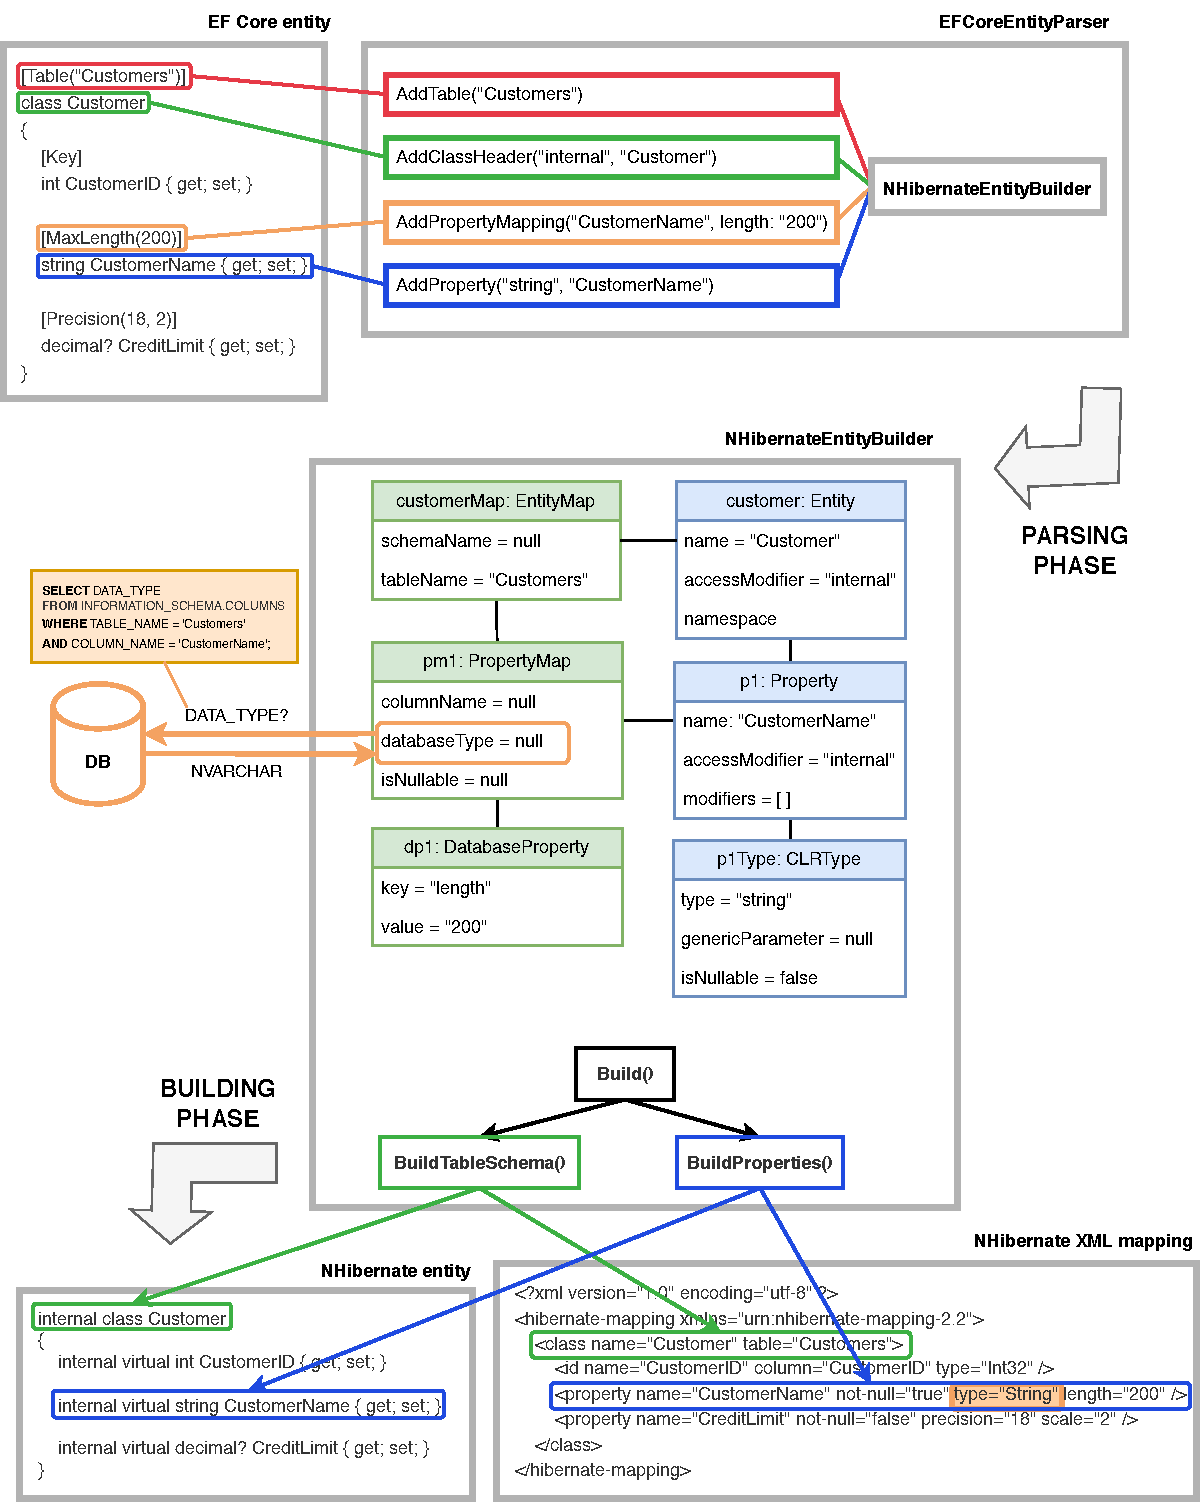
\includegraphics[width=\textwidth]{thesis/img/thesis/03_parsing_building.drawio.pdf}
  \caption{Translation of \acrshort{ef} Core entity mapping to NHibernate.}
  \label{fig:translation_complete}
\end{figure}

% maybe TODO builder pseudocode